\newpage

\section{Building a Pedometer using an Accelerometer}
\label{s:pendulum}

\subsection{Parts List}

\begin{enumerate}[itemsep=-5pt]
\item Laptop
\item CPX/CPB
\item USB Cable
\item External Battery Pack
\end{enumerate}

\subsection{Learning Objectives}
\begin{enumerate}[itemsep=-5pt]
\item Understand how to run CPB/CPX while not tethered to a computer
\item Reinforce bluetooth tech for data transfer
\item Understand post-processing for debugging to be used for online calculations
\item Understand the fundamentals of how a pedometer works
\end{enumerate}

\subsection{Getting Started}

A pedometer is a device that counts the number of steps. Typically
these are worn as watches with popular brands like Garmin or Fitit
owning the market share at the time of this writing. It turns out
though that your phone and apps like Google Fit can also track steps
just by being inside your pocket all day. The way they do this is by
measuring the acceleration, angular velocity and potentially even the
angles (using a magnetometer) to count steps. In this lab this we will
just focus on attempting to get steps using accelerometer data.  

\subsection{Gathering Accelerometer Data}

First we need to make sure we can gather accelerometer data. The low
level accelerometer code is relatively simple and is explained in the
Modules lab (Section \ref{s:Modules}). In order to gather the
accelerometer data while running you'll need to be able to operate the
CPB/CPX untethered from a computer. This means you have to use Method
3 or 4 (Section \ref{s:daq} and \ref{s:Bluetooth}). Remember that
Method 1 and 2 require a computer and running with a computer would be
difficult. Method 3 requires a lot of setup to log data directly to
the disk so for this lab we will just use the Bluetooth module to send
data directly to your phone. Note that if you have a CPX you will have
to use Method 3. The best way to do this experiment is with a
partner. Have the CPB/CPX measure acceleration and place the entire
device with a battery pack inside the runners pocket. Then have your
partner connect to the CPB with the Adafruit Connect app and log
data using the UART and Export to txt function. Remember not to run
too far because the Bluetooth signal distance is only about 30
feet. See if you can combine the Bluetooth code and the acceleration
code into one code to send time and the 3-axis accelerometer data. If
you're still having trouble, code for this lab can be found
on \href{https://github.com/cmontalvo251/Microcontrollers/tree/master/Circuit_Playground/CircuitPython/pedometer}{Github}. Note
if you have a CPX you will need to combine the accelerometer code with
the Method 3 version of data logging.

Running the CPX/CPB untethered does require a few extra steps besides
writing the code. The first step is obviously to write the software
that you want to run on the CPX/CPB. I recommend testing the code
extensively while tethered to the computer so you can debug using the
REPL. Once you're certain the code works you can disconnect the
CPX/CPB and connect it to a battery pack. Once again I recommend
testing the code with the battery back before you perform the
experiment. In this experiment I used an external USB battery bank as
shown in the photo below. My code also utilizes the neopixel library
to turn on some LEDs. 
\begin{figure}[H]
  \begin{center}
    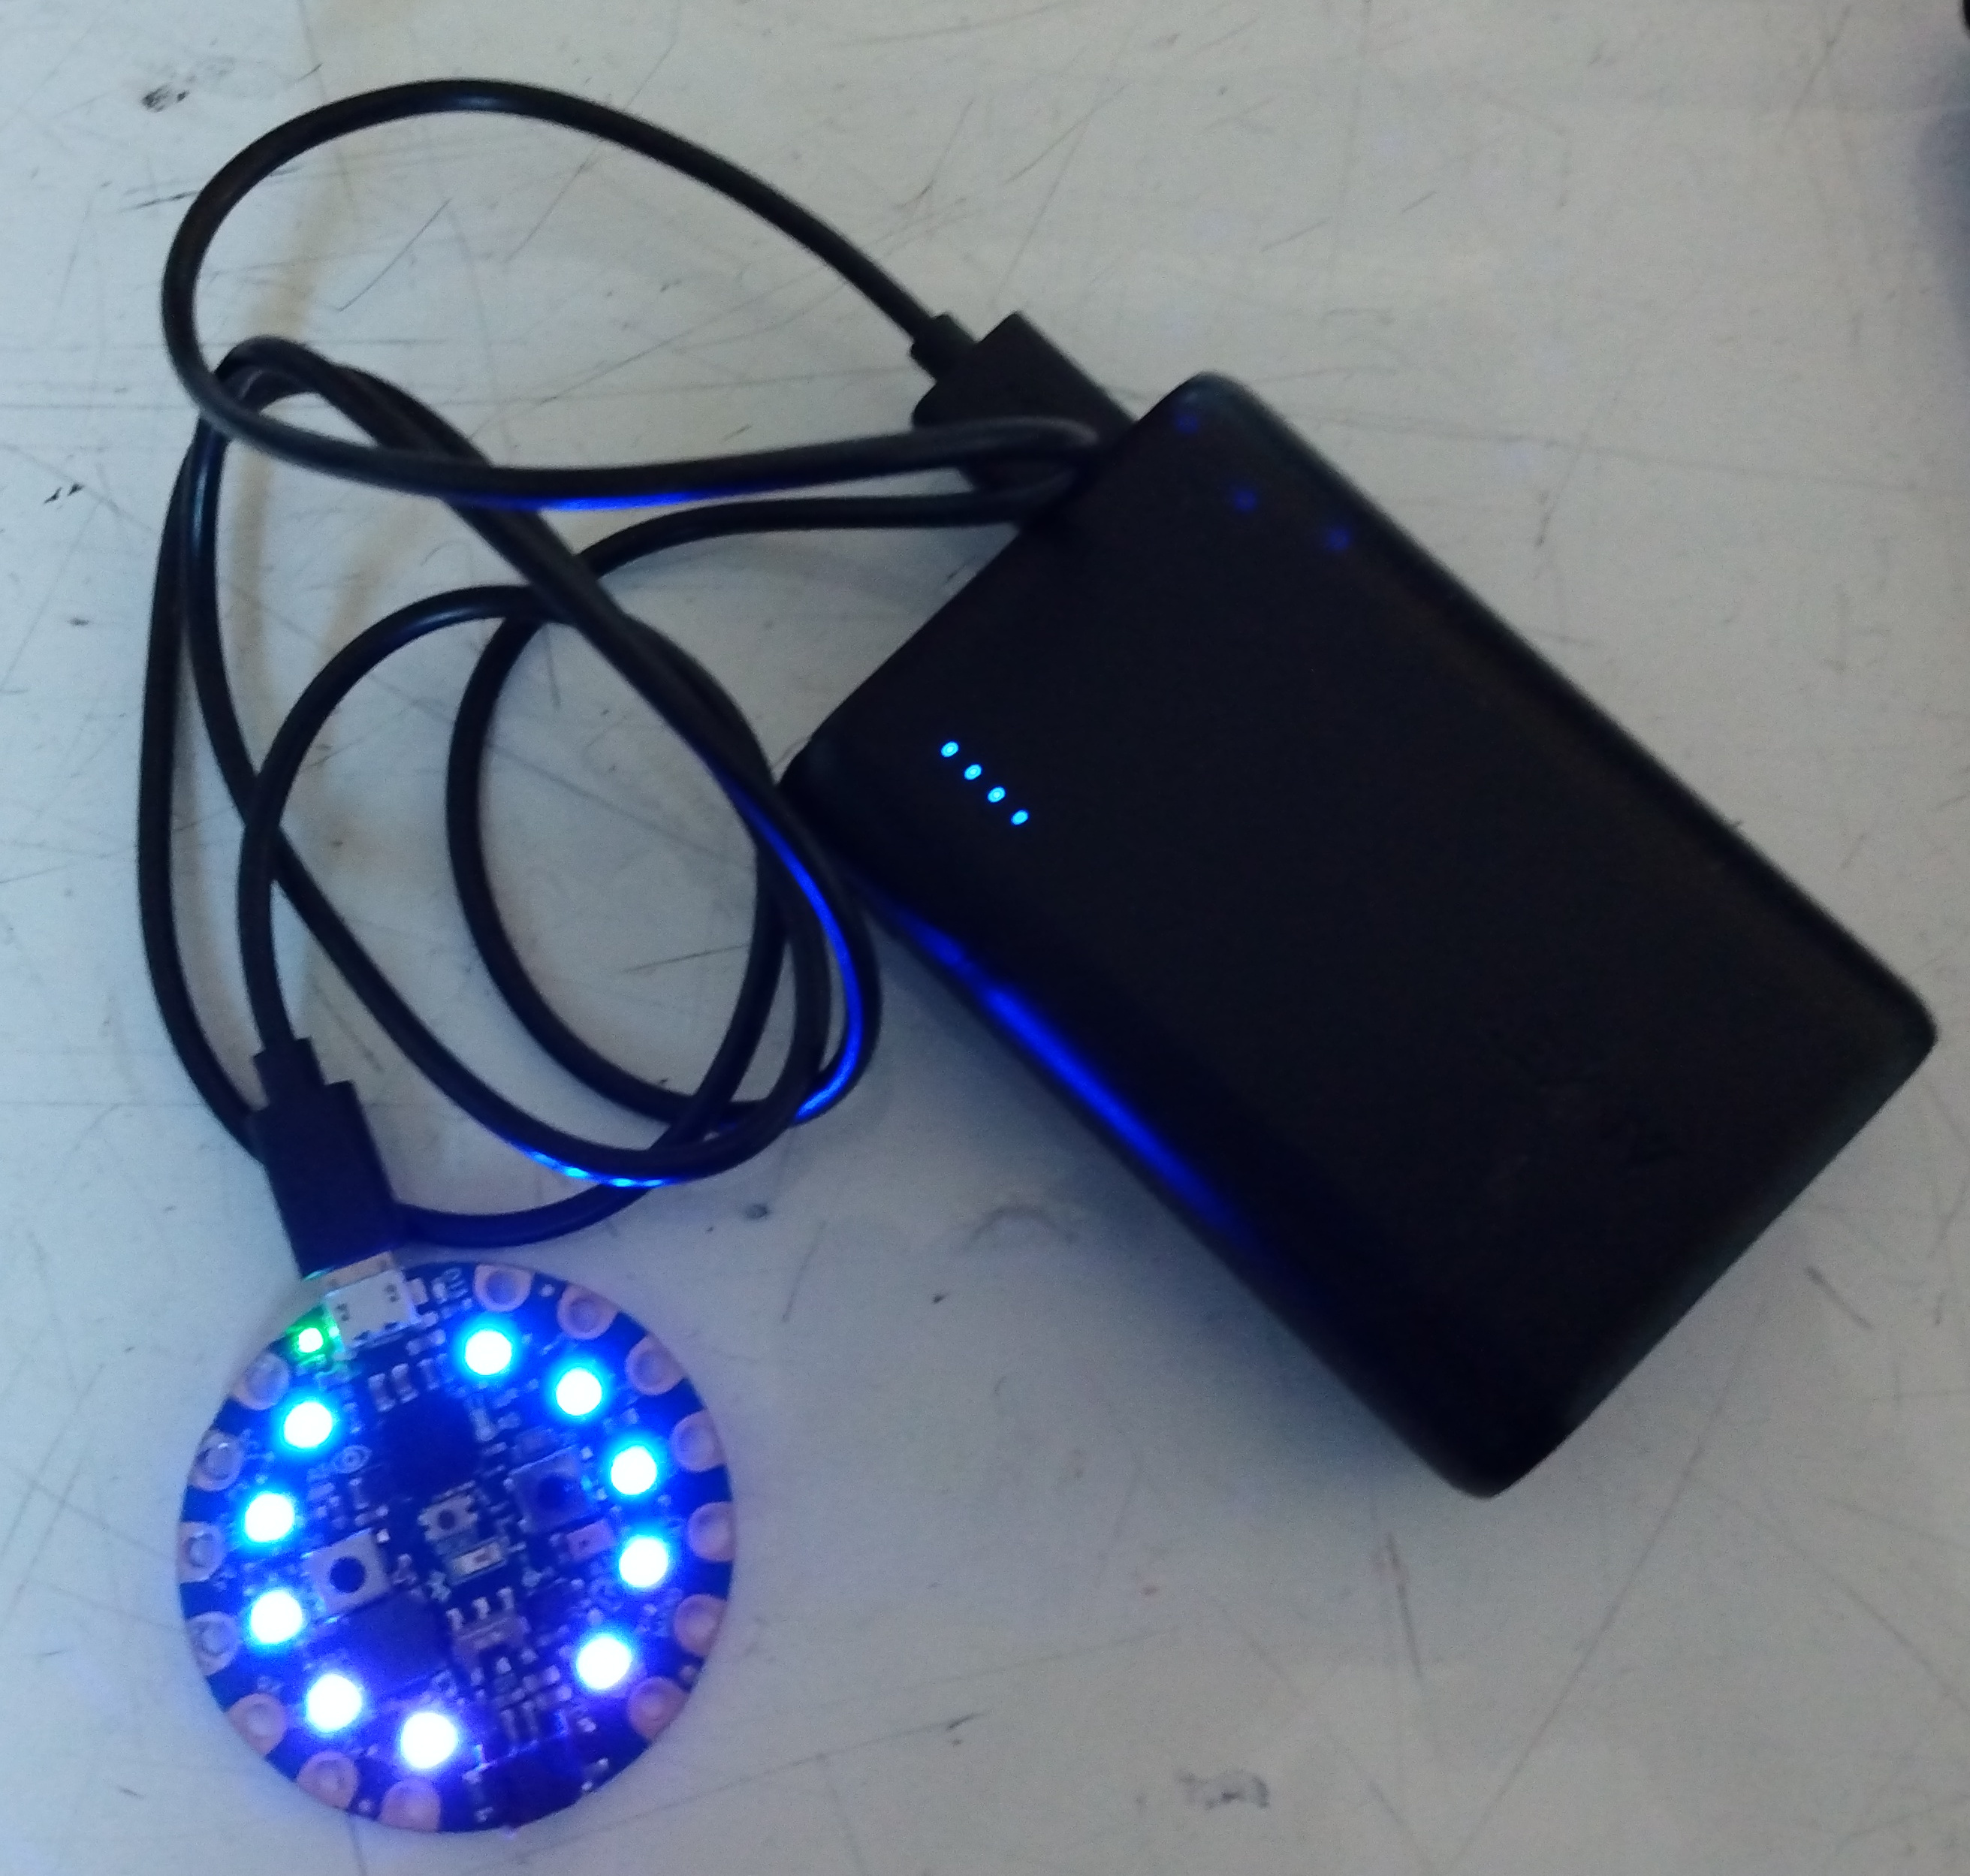
\includegraphics[width=0.8\textwidth]{Figures/External_Battery_Pack.jpg}
  \end{center}
\end{figure}

\subsection{Computing Number of Steps: Post-Processing}

Using the hardware and software defined above I had my partner run down the hallway after I ensured there was a solid connection between the CPB and my smart phone. I then exported the data to a text file and plotted the raw data using Thonny. 
\begin{figure}[H]
  \begin{center}
    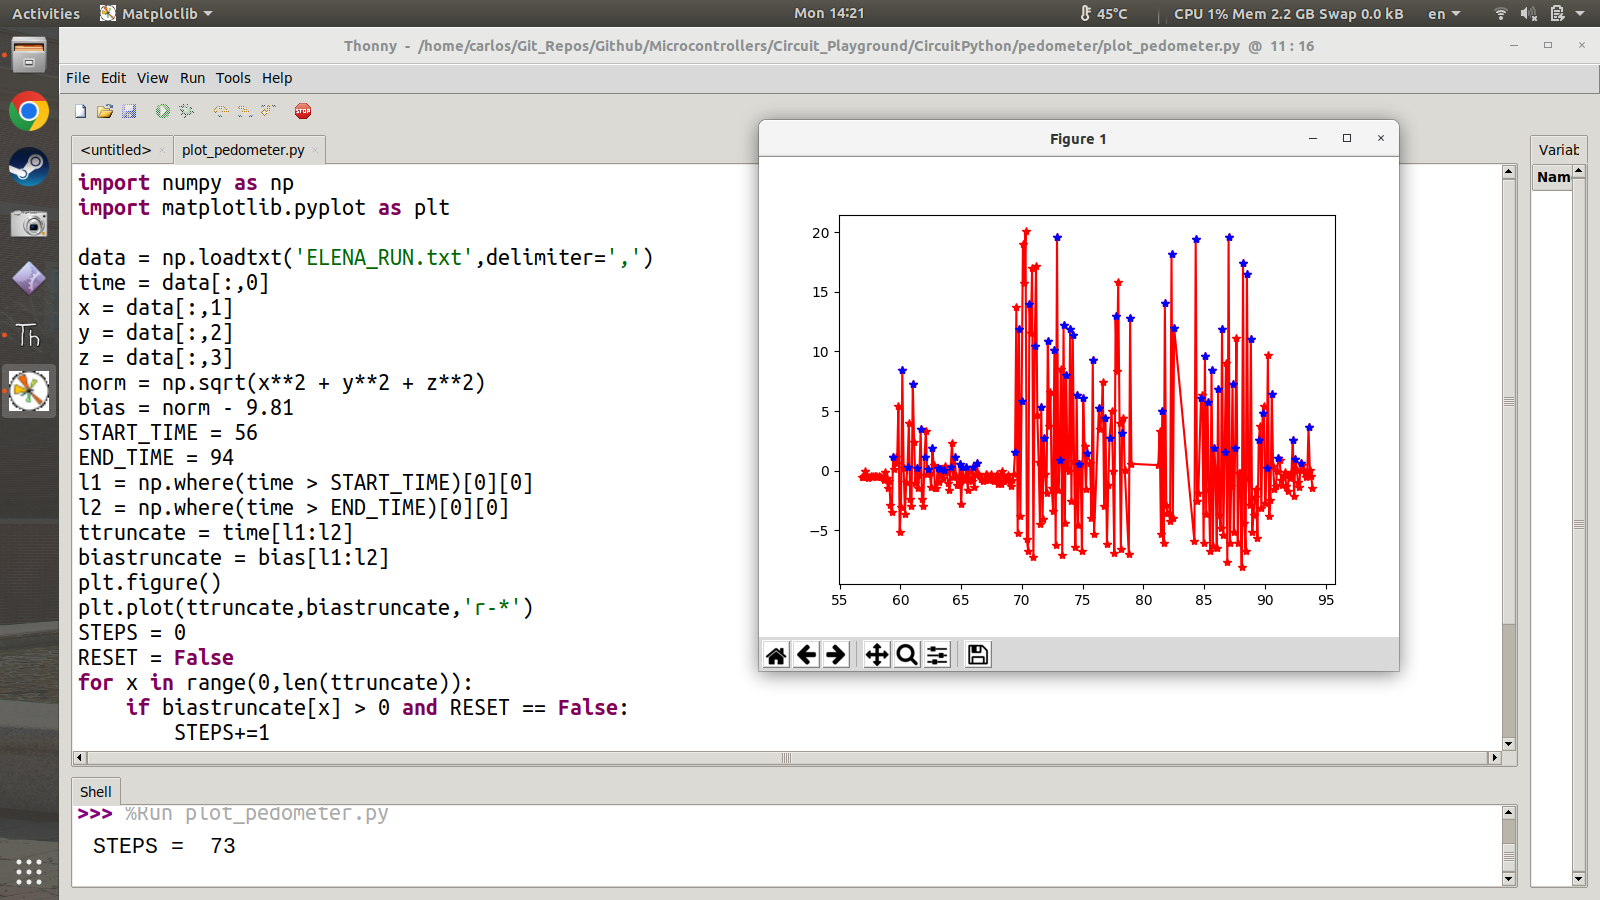
\includegraphics[width=\textwidth]{Figures/Pedometer3.png}
  \end{center}
\end{figure}
Upon inspecting the raw data it seems as though my partner began running around 68 seconds. At about 80 seconds my partner reached the end of the hallway and the CPB got a bit out of range. As such there is a gap in the data. The accelerometer streams return once my partner begins running back down the hallway. In order to simply look at the data of one run the data was truncated from 69 seconds to 79 seconds as shown in the Figure below.
\begin{figure}[H]
  \begin{center}
    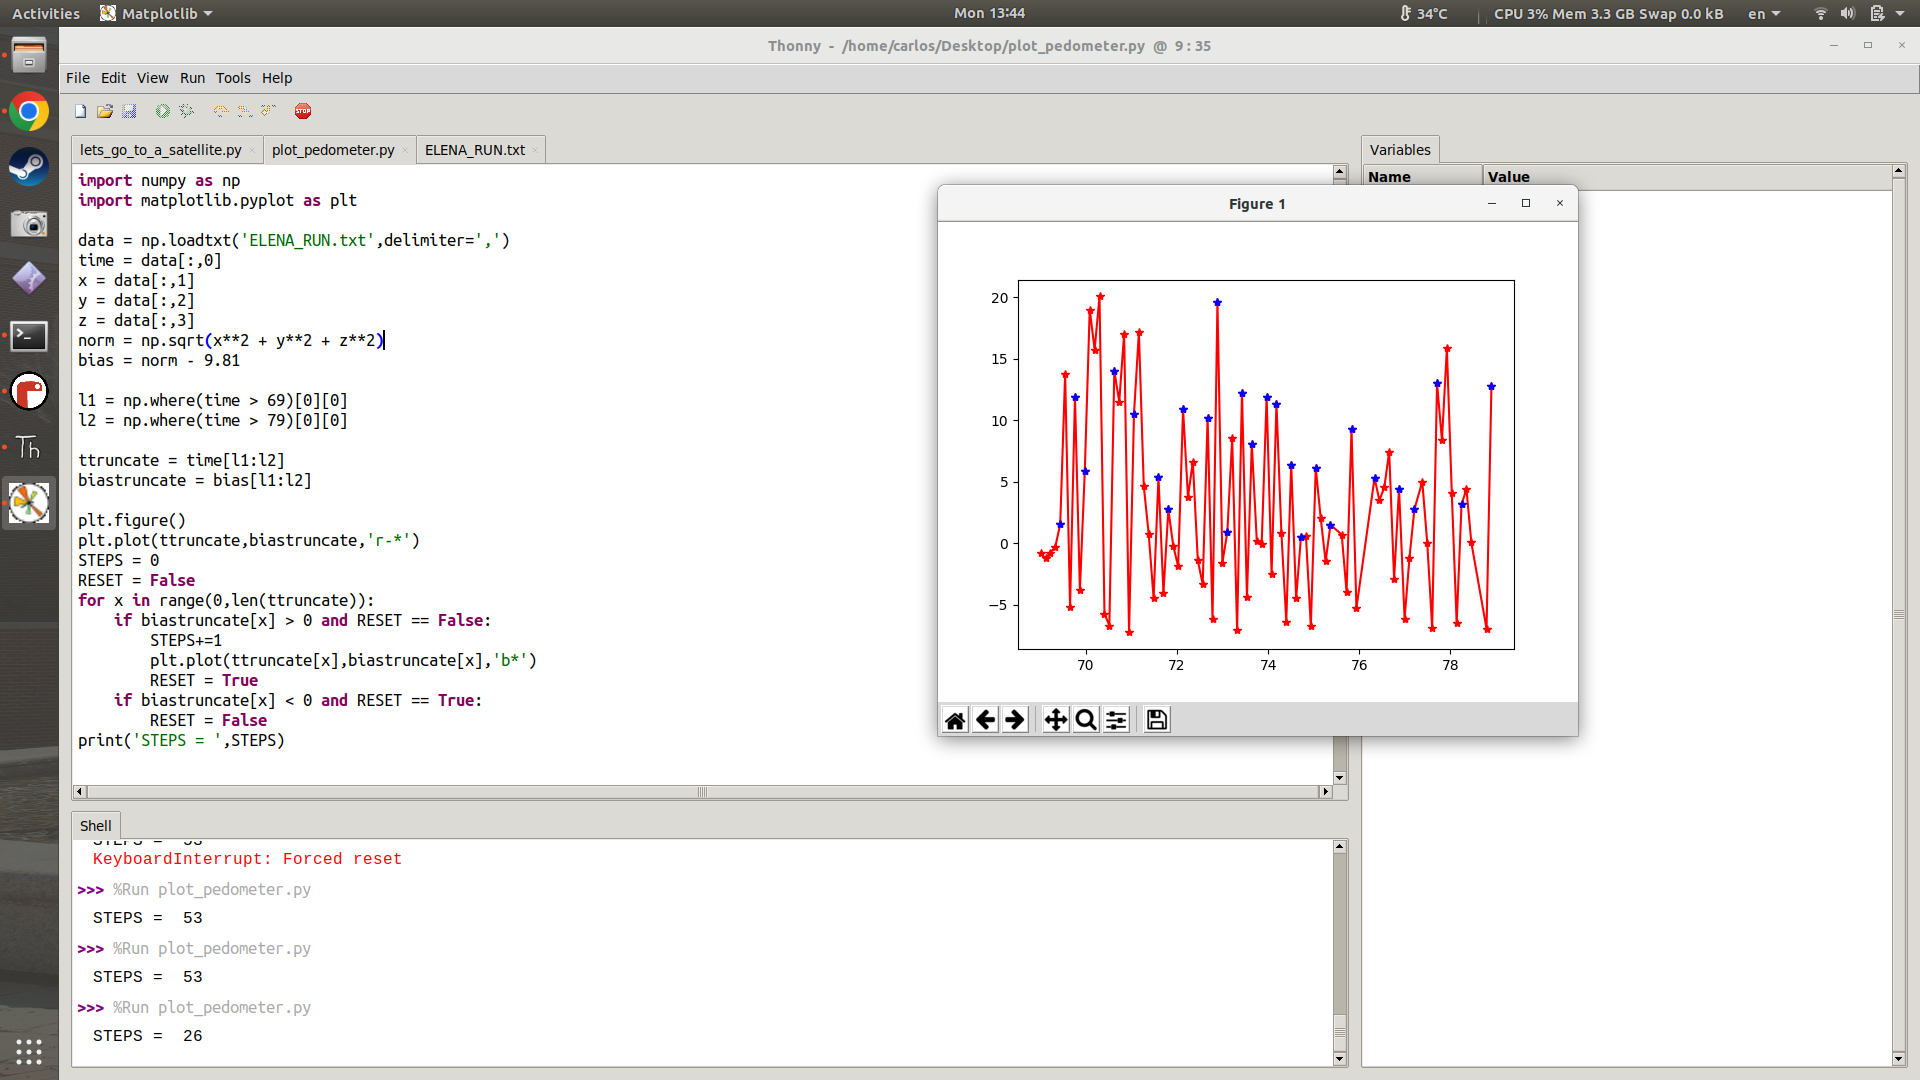
\includegraphics[width=\textwidth]{Figures/Pedometer2.png}
  \end{center}
\end{figure}
In order to count steps the algorithm is fairly simple and not very robust but it does at least give you a sense of how data can be analyzed to obtain steps. First, the norm of the accelerometer data is computed and then the norm is substracted by 9.81 $m/s^2$. When glancing at the data the steps seem to be taken when the result of the norm-9.81 goes from positive to negative. It is possible that there is some aliasing in the data but for a simple experiment like this a rudimentary algorithm can be created. First the STEP counter is set to zero and then a for loop is created to loop through the data. When the data goes from positive to negative a STEP is created. This is done by using a RESET flag and checking whether or not the data becomes positive. This algorithm computes 26 steps which seems reasonable for the length of the hallway.

\subsection{Computing Number of Steps: Online}

The benefit of post-processing in Python is that the CPX/CPB run a almost identical derivative of Python called CircuitPython. This means that almost any line of code used in Python can be copied directly onto the CPX/CPB as shown in the Figure below.
\begin{figure}[H]
  \begin{center}
    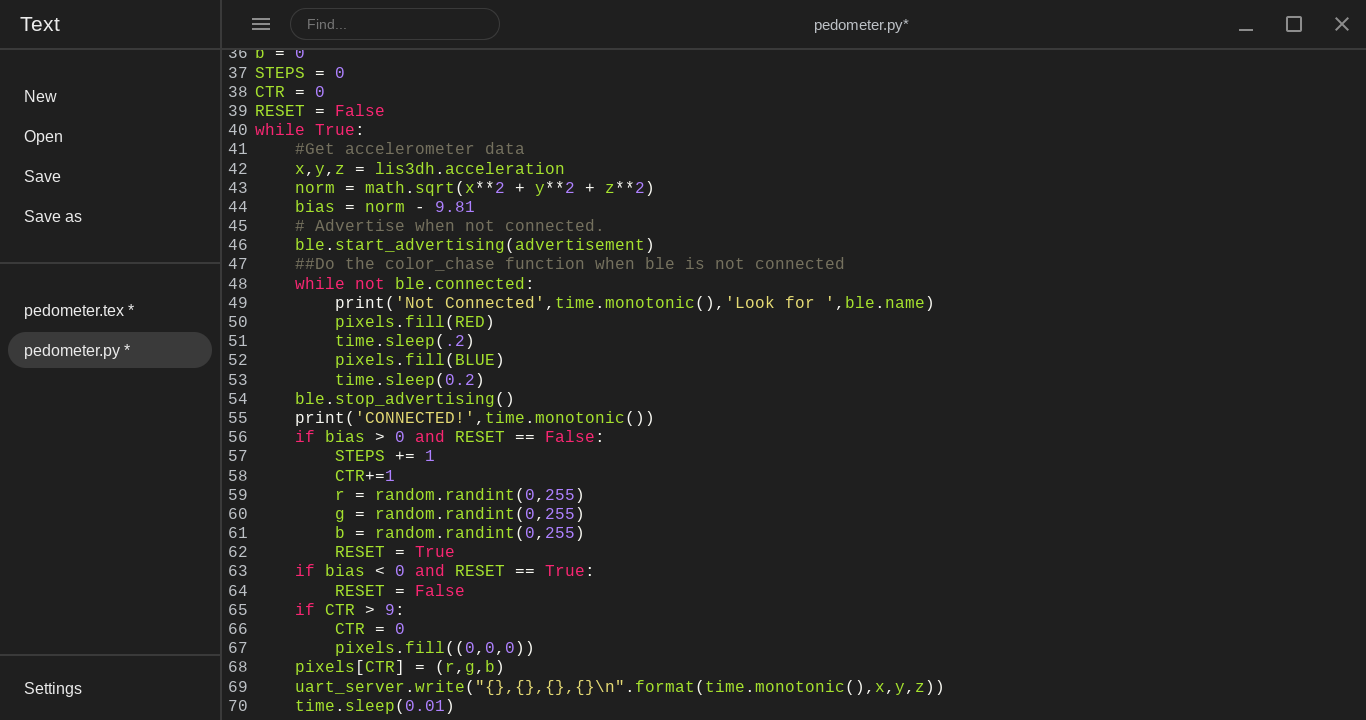
\includegraphics[width=\textwidth]{Figures/Pedometer4.png}
  \end{center}
\end{figure}
You can see that the STEPS counter is set to zero before the infinite while loop and then after connection the RESET flag and bias value are checked for a switch from positive to negative. Some code is added to change the pixels on the CPB so that the user can see a step change. The raw data is still transmitted via bluetooth but it would be a neat exercise to have the CPB transmit the number of steps to a cell phone for instant feedback of the number of steps. 

\subsection{Assignment}

Upload a PDF with all of the photos and text below included. My recommendation is for you to create a Word document and insert all the photos and text into the document. Then export the Word document to a PDF. For videos I suggest uploading the videos to Google Drive, turn on link sharing and include a link in your PDF.

\begin{enumerate}[itemsep=-5pt]
\item Include a video of you gathering accelerometer data via bluetooth - 30\%
\item Include a video of your partner running down the hallway. How many steps did they take? - 30\%
\item Include a plot of accelerometer data and how many steps your partner took according to the accelerometer data - 30\%
\item Compare the results from the accelerometer data and the actual number of steps in the video. Are they the same? Different? Why or why not? - 10\%
\end{enumerate}
